\documentclass[a4paper,oneside,DIV=12,12pt,headings=normal]{scrartcl}

%%% Length calculations
\usepackage{calc}
%%%

%%% Support for color
\usepackage{xcolor}
\definecolor{lightblue}{HTML}{03A9F4}
\definecolor{red}{HTML}{F44336}
%%%

%%% Graphics inclusion
\usepackage{graphicx}
%%%

%%% Font selection
\usepackage{fontspec}

\setromanfont{STIX Two Text}[
]

\setsansfont{Source Sans Pro}[
]

\setmonofont{Source Code Pro}[
]

\usepackage{amsmath,unicode-math}
\setmathfont{STIX Two Math}

%%%

%%% Font settings for different KOMA Script elements
\setkomafont{pagenumber}{\rmfamily}
\setkomafont{disposition}{\rmfamily\bfseries}
%%%

%%% Typographic enhancements
\usepackage{microtype}
%%%

%%% Language-specific settings
\usepackage{polyglossia}
\setmainlanguage{ukrainian}
%%%

%%% List settings
\usepackage{enumitem}
\setlist[enumerate]{
	leftmargin = *,
}
%%%

%%% Captions
\usepackage{caption}
\usepackage{subcaption}

\DeclareCaptionLabelFormat{closing}{#2)}
\captionsetup[subtable]{labelformat = closing}
\captionsetup[subfigure]{labelformat = closing, position = auto}
%%%

%%% Tables
\usepackage{booktabs}
\usepackage{longtable}

\usepackage{multirow}

\usepackage{array}
\newcolumntype{v}[1]{>{\raggedright\arraybackslash\hspace{0pt}}p{#1}}
\newcolumntype{b}[1]{>{\centering\arraybackslash\hspace{0pt}}p{#1}}
\newcolumntype{n}[1]{>{\raggedleft\arraybackslash\hspace{0pt}}p{#1}}
%%%

%%% Links and hyperreferences
\usepackage{hyperref}
\hypersetup{
	colorlinks      = false,
	linkbordercolor = red,
	urlbordercolor  = lightblue,
	pdfborderstyle  = {/S/U/W 1.5},
}
%%%

%%% All caps
\newcommand{\allcaps}[1]{{\addfontfeatures{LetterSpace = 3}#1}}
%%%


\begin{document}
	\begin{titlepage}
	\centering
		Міністерство освіти і науки України\\
		Національний авіаційний університет\\
		Навчально-науковий інститут комп'ютерних інформаційних технологій\\
		Кафедра комп'ютеризованих систем управління

		\vspace*{\fill}

		Лабораторна робота №3\\
		з дисципліни «Архітектура комп'ютерів»\\
		на тему «Побудова блоку обробки даних»\\
		Варіант №4

		\vspace*{\fill}
		
		\begin{flushright}
			Виконав:\\
			студент ННІКІТ СП-225\\
			Клокун В.\,Д.\\
			Перевірив:\\
			Зіньков Ю.\,Г.
		\end{flushright}

		Київ 2018
    \end{titlepage}
	
	\section{Мета роботи}
		Вивчення схемотехніки та системи мікрооперацій процесорного елементу~К1804ВС1, побудова блоку обробки даних на його основі та розробка мікропрограм обчислення функцій.
		
	\section{Хід роботи}
		Розроблюємо алгоритм для блоку обробки даних та записуємо його у вигляді блок-схеми~(рис.~\ref{fig:algorithm}).
		\begin{figure}[!htbp]
		\centering
			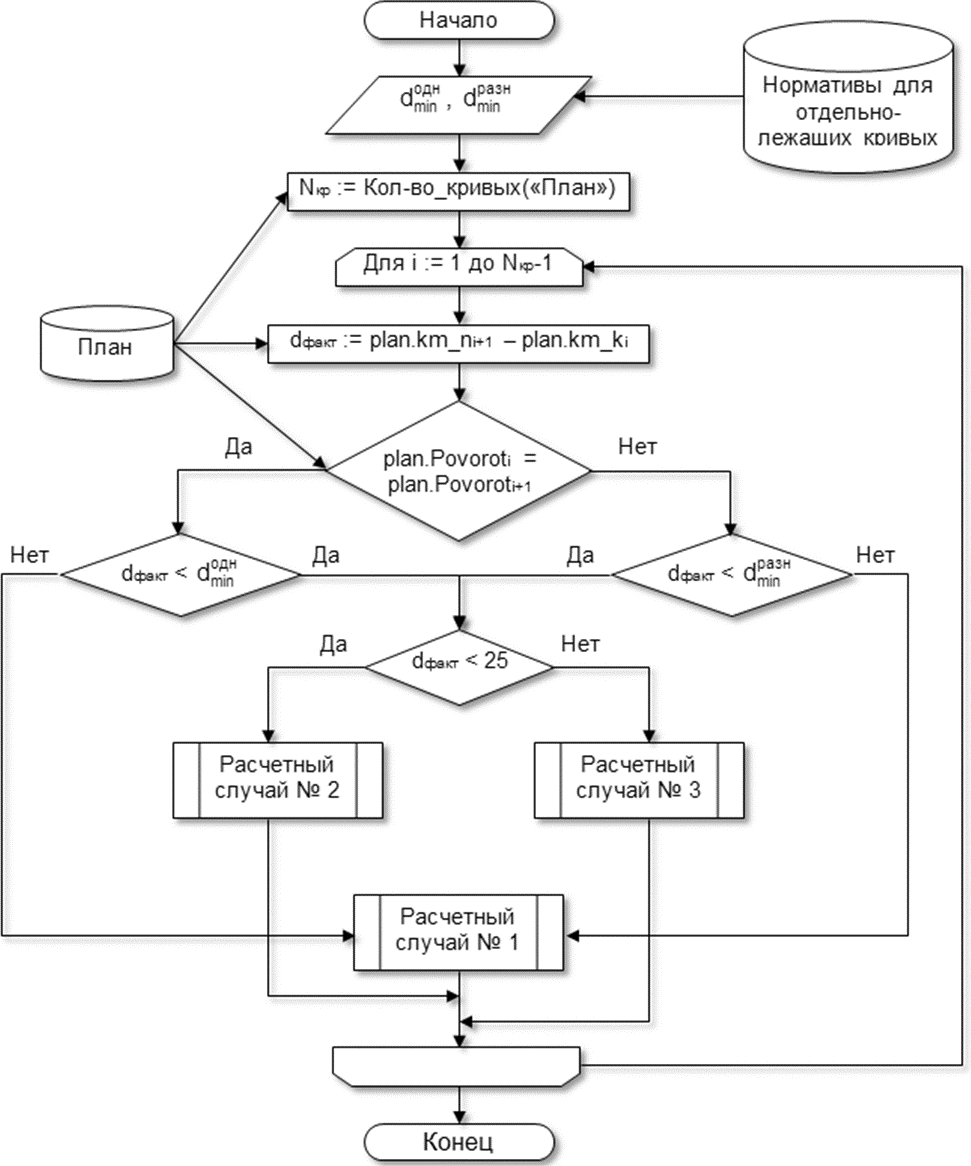
\includegraphics[height = 30\baselineskip]{./assets/00.png}
		\caption{Алгоритм для блоку обробки даних}
		\label{fig:algorithm}
		\end{figure}
		
		На основі розробленого алгоритму будуємо арифметично-логічний пристрій і~зображуємо його у вигляді принципової схеми~(рис.~\ref{fig:alu}).
		\begin{figure}[!htbp]
		\centering
			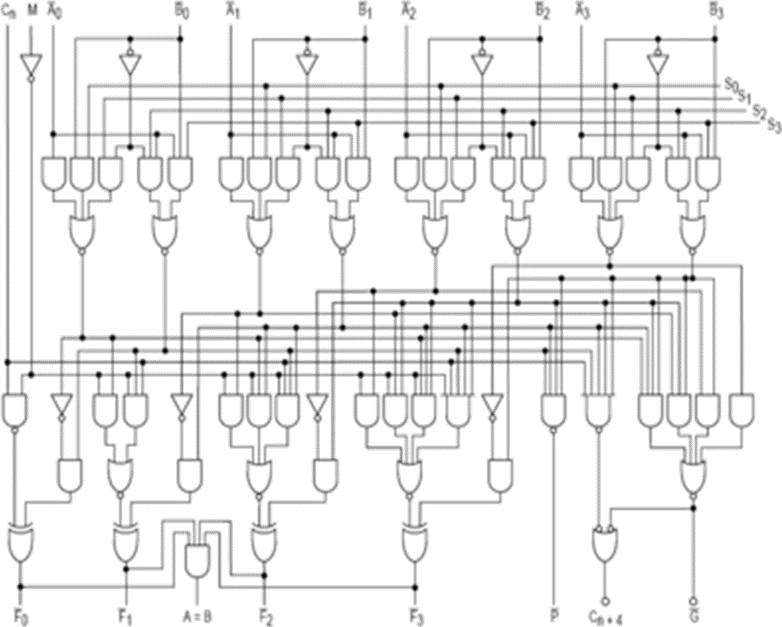
\includegraphics[height = 15\baselineskip]{./assets/01.png}
		\caption{Схема арифметично-логічного пристрою}
		\label{fig:alu}
		\end{figure}
		
		Моделюємо роботу розробленого алгоритму та отримуємо результати~(табл.~\ref{tab:results}).
		
		\begin{table}[!htbp]
		\centering
			\begin{tabular}{lb{2.5em}b{2.5em}b{2.5em}b{2.5em}ll}
				\toprule
					№~стану & \multicolumn{4}{c}{Набір керуючих сигналів} & $M = 1$ & $M = 0$ \\
					\cmidrule(lr){2-5}
					 & $S_3$ & $S_2$ & $S_1$ & $S_0$ & & \\
				\midrule
					0 & 0 & 0 & 0 & 0 & $\neg A_i$ & $A + C_0$ \\
					1 & 0 & 0 & 0 & 1 & $\neg (A_i \lor B_i)$ & $(A \lor B) + C_0$ \\
					2 & 0 & 0 & 1 & 0 & $\neg A_i \cdot B_i$ & $(A \lor \neg B) + C_0$ \\
					3 & 0 & 0 & 1 & 1 & $0$ & $2^4 - 1 + C_0, 0 \text{ при } C_0 = 1$ \\
					4 & 0 & 1 & 0 & 0 & $\neg (A_i \cdot B_i)$ & $A + (A \land \neg B) + C_0$ \\
					5 & 0 & 1 & 0 & 1 & $\neg B_i$ & $(A \lor B) + (A \land \neg B) + C_0$ \\
					6 & 0 & 1 & 1 & 0 & $A_i + B_i$ & $A - B - 1 + C_0$ \\
				\bottomrule
			\end{tabular}
		\caption{Результати моделювання}
		\label{tab:results}
		\end{table}
		
	\section{Висновок}
		Виконуючи дану лабораторну роботу, ми ознайомились зі схемотехнікою та системою мікрооперацій процесорного елементу~К1804ВС1; побудували блок обробки даних на його основі та розробили мікропрограму обчислення функції.
\end{document}